\documentclass{article}
\usepackage[utf8]{inputenc}
\usepackage{hyperref}
\usepackage{url}
\usepackage{amsmath}
\usepackage{tikz}
\usetikzlibrary{positioning, calc, arrows.meta}

\title{Decentralised Voting}
\author{Errol Drummond\\ \texttt{Aleo, Dock}\\ \and 
 Luke Pearson\\ \texttt{Polychain Capital} \and
 Thomas Norton \\ Webb}
\date{November 2021}

\begin{document}

\maketitle
\section{Abstract}
This is a decentralised voting system built for secure, privacy-preserving participation amongst multiple anonymous parties. The decentralisation of the tallying procedure is a novel addition to voting infrastructure. Of particular interest is that this setup allows the MPC to use a single public key to publish the vote's result, to publish data on the voting chain from another chain using this public key, or publish on another chain using a distributed key. If you want to discuss anything about this design, join the telegram group \href{https://t.me/joinchat/5tZhfUWRwacwNzZk}{here}.

\section{Introduction}
This design aims to be as safe as MACI (the properties MACI tries to achieve are listed at the end), but make the vote tallying process decentralised. There will still be the organisation the vote is for (henceforth referred to as O), and they have a few roles:
\begin{enumerate}
    \item Maintain the list of eligible voters
    \item Send the voter's 'voting point' $g_i$ (if preferred, voters could choose these points themselves and send them to O)
    \item There will be an initial setup ceremony (an arbitrary number of elections can be held after this), and O may or may not be involved in this
\end{enumerate}

This infrastructure is paramount to the developing DAO space, and to decentralised governance in general. Aside from the novel addition of a dencentralised tallying mechanism, the design also allows for easy addition of keys on other chains. This will allow the MPC committee to publish things on other chains without a bridge, and also to publish things on the voting chain from other chains (also to publish the result of the vote on chain too)

This works under the paradigm of ZEXE, so the native on-chain transaction is a proof of validity of an off chain computation; all records are private by default. ZEXE is implemented by Aleo, an L1 for privacy centered, scalable applications. The default privacy is essential to this design.

\section{Preliminaries}
\subsection{Accumulators}
We will need to make use of a positive accumulator; this will serve as both a whitelist for eligible voters, and also provide structure we need for the vote. The accumulator is published at the start of the vote and does not need to be updateable.

\subsection{Encryption schemes}
The encryption schemes used here will be of a threshold type, a brief description of which can be found in the appendix.

There will be three unique private keys, $s_1$, $s_2$ and $s_3$, shared among the MPC committee. These 3 secret keys will be used to create 2 public scalar points, $s_1P$ and $s_2P$, and 3 secret keys, $s_2s_3$, $s_1s_3$ and $s_3$ - after this the shards of the original public keys, $s_1$ and $s_2$, should be erased.

One point to elaborate on is that, if we have some other scalar $r$, we can create both $rs_1P$ and $rs_2P$, but we cannot create $rs_1s_2P$ without using the MPC committee. This will be relevant later, because the committee will generate $rs_1s_2s_3P$, but since no voter can generate it it will be impossible to link tallied votes to the voters who sent them.

\subsection{Vote representation}
Votes will be determined in a graph theoretic way. Voters will be have some value $g_i$. Voters will send records that are only valid if they 'point' to their own value $g_i$ (by blinding $g_i$ with a couple random scalars, chosen differently with the creation of each record). 

If there are $k$ vote options in the vote, then the voter's vote is determined by the number of records they have pointing to their $g_i$. If there are 3 options, and the number of records pointing at their $g_i$ is $m$, we have option 1 if $m\equiv1\bmod3$, option 2 if $m\equiv2\bmod3$, and option 0 if $m\equiv0\bmod3$.

It is up to the users of this system to decide whether they want to include a `null` vote option to signal discontent.

\section{Protocol}
\subsection{One-time setup}
There is a need for encryption/decryption keys to be shared among sets of nodes; this is where we are decentralising the role of the trusted central party.

The nodes who will be sharing the keys will run a non-interactive distributed key generation and key resharing protocol such as  \href{https://eprint.iacr.org/2021/339.pdf}{Groth} or \href{https://eprint.iacr.org/2021/1397.pdf}{GHL}. All nodes that are going to be involved will run an MPC wherein the encryption/decryption keys are generated, and the relevant keys sharded and shared among the nodes.

\subsection{Setup}
O will publish a whitelist accumulator of eligible voters. Elements of this whitelist contain two things:
\begin{enumerate}
    \item The public key of the eligible voter.
    \item Some random scalar $g_i$ that is unique to the voter.
\end{enumerate}

When sending records, voters will prove both that they are eligible to vote, and that their vote 'points' to their $g_i$ value.

When publishing this accumulator, O will also send a record to each eligible voter that contains their $g_i$ value (essentially encrypted communication); alternatively, eligible voters could send the accumulator their $g_i$ value directly.

Alternatively, the accumulator of valid voters could also be maintained in a more decentralised manner, such as having a specific set of rules for allowing public keys to be added or removed.

\subsection{Voting}
We will refer to the thing being created by voters as `nodes'. This terminology is used because we can think of the voters as building a star shaped tree. In the center of the tree will be the voter's scalar $g_i$, and the voter adds nodes that `point' to the center - you can see this more clearly in figure \ref{fig:figure1}. For each node created, the voter will produce 2 random scalars, $r_{i,j,1}$ and $r_{i,j,2}$; the $i$ represents the voter, and the $j$ represents which node is being referenced. In these nodes (which are published as records in the ZEXE model), the voter has to input several things:
\begin{enumerate}
    \item A message saying this is a vote in vote X.
    \item A proof that they are eligible to vote, and that when they use $g_i$, it is the correct value (i.e. the one in the accumulator associated with their name).
    \item A double blinded reference to their unique value, $g_iP + r_{i,j,1}s_1P + r_{i,j,2}P$.
    \item A shielded reference to their blinding values, $r_{i,j,1}s_2P$ and $r_{i,j,2}s_2P$. The MPC committee will later use these to determine $r_{i,j,1}s_1s_2s_3P$, $r_{i,j,2}s_2s_3P$, and unshield the pointer.
\end{enumerate}

\begin{figure}[h!]
        \centering
        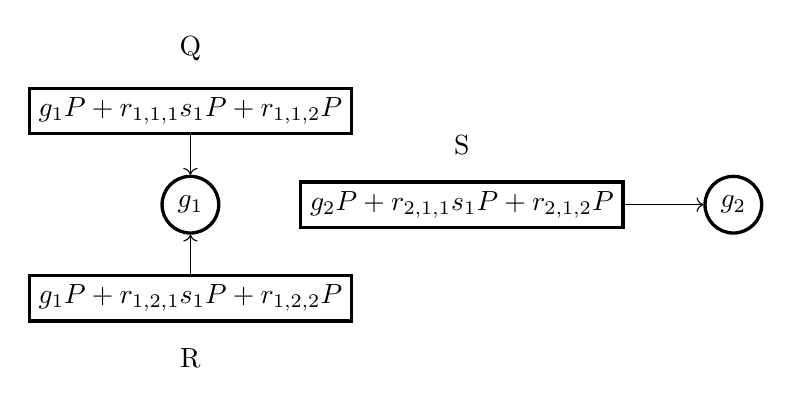
\begin{tikzpicture}
    [roundnode/.style={circle, draw=black, very thick},
    squarednode/.style={rectangle, draw=black, very thick},]


    %Nodes
    \node[squarednode](Q){$g_1P+r_{1,1,1}s_1P + r_{1,1,2}P$};
    \node[roundnode](G1)[below=0.5cm of Q]{$g_1$};
    \node[squarednode] (R)[below=0.5cm of G1] {$g_1P+r_{1,2,1}s_1P + r_{1,2,2}P$};

    \node[squarednode](S)[right=of G1]{$g_2P+r_{2,1,1}s_1P + r_{2,1,2}P$};
    \node[roundnode](G2)[right=of S]{$g_2$};

    %Lines
    \draw[->](Q.south)--(G1);
    \draw[->](R.north)--(G1);
    
    \draw[->](S.east)--(G2);

    %Labels
    \node(Qlabel)[above=0.2cm of Q]{Q};
    \node(Rlabel)[below=0.2cm of R]{R};
    \node(Slabel)[above=0.2cm of S]{S};
    
\end{tikzpicture}

        \caption{A representation of the voting trees being constructed, though the connections between the nodes cannot be seen on chain.}
        \label{fig:figure1}
\end{figure}

\begin{figure}[h!]
        \centering
        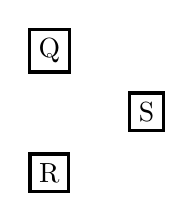
\begin{tikzpicture}
    [roundnode/.style={circle, draw=black, very thick},
    squarednode/.style={rectangle, draw=black, very thick},]

    %Nodes
    \node[squarednode](Q){Q};        
    \node[squarednode](R)[below=1cm of Q]{R};
    \node[squarednode] (S)[right=1cm of {$(Q)!0.5!(R)$}] {S}; 
\end{tikzpicture}

        \caption{This is what observers actually see during the vote; they only see that nodes are being added, not any of the edges connecting nodes. These 3 nodes could all be from separate voters, or they could all be from the same voter - there is nothing we can realistically do to know.}
        \label{fig:figure2}
\end{figure}

Due to the private nature of the ZEXE design, it will be impossible to see who is sending nodes - figure \ref{fig:figure2} represents what is actually visible to a general observer. However, any voter is free to uncover any of the nodes they wish to a potential briber (by giving them the pre-images of the above items); but voters can show any subset of the tree of nodes they are making, and thus 'prove' they voted however they wish. Hence a 'proof' of how one voted is meaningless.

\subsection{Vote tallying}
When the vote is over, the MPC committee will batch the nodes into small enough batches such that it will be computationally feasible to conduct the MPC.

For each batch, the MPC member will do 3 things (and also produce a proof that these things were all done correctly). The MPC member will do something locally to each node, and they will also do something globally to the set of nodes in their batch - you can look at figure \ref{fig:figure3} for a visual of the local change, and at figure \ref{fig:figure4} for a visual of the global change:
\begin{enumerate}
    \item Apply their shard ($s_{2,k}s_{3,k}$) of $s_2s_3$ to $g_iP+r_{i,j,1}s_1P + r_{i,j,2}P$.
    \item Apply their shard ($s_{1,k}s_{3,k}$) of $s_1s_3$ to $r_{i,j,1}s_2P$.
    \item Apply their shard ($s_{3,k}$) of $s_3$ to $r_{i,j,2}s_2P$.
    \begin{figure}[h!]
        \centering
        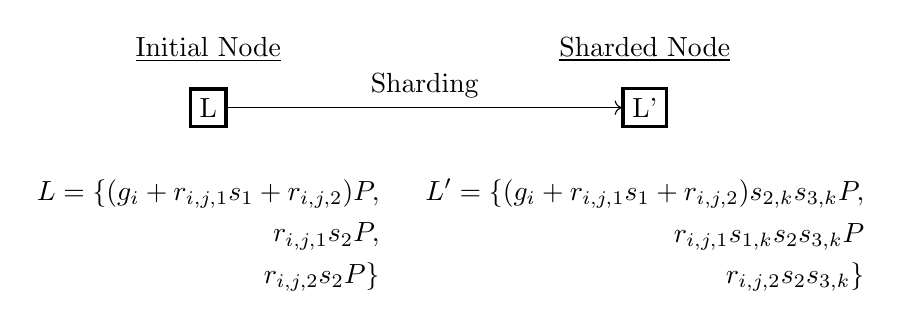
\begin{tikzpicture}
    [roundnode/.style={circle, draw=black, very thick},
    squarednode/.style={rectangle, draw=black, very thick},]

    %Nodes
    \node[squarednode](L1){L};        
    \node[squarednode](L2)[right=5cm of L1] {L'};

    %Labels
    \node(intialnode)[above=0.2cm of L1]{\underline{Initial Node}};
    \node(shardednode)[above=0.2cm of L2]{\underline{Sharded Node}};

    %Lines
    \draw[->](L1)--node[above]{Sharding}++(L2);

    %Equations
    \node(L1equation)[below=0.5cm of L1]{
        $\begin{aligned}
            L=\{(g_i+r_{i,j,1}s_1+r_{i,j,2})P, \\ r_{i,j,1}s_2P, \\ r_{i,j,2}s_2P\}
        \end{aligned}$
        };
    \node(L2equation)[below=0.5cm of L2]{
        $\begin{aligned}
            L'=\{(g_i+r_{i,j,1}s_1 + r_{i,j,2})s_{2,k}s_{3,k}P, \\r_{i,j,1}s_{1,k}s_2s_{3,k}P \\ r_{i,j,2}s_2s_{3,k}\}
        \end{aligned}$
        };
    
\end{tikzpicture}

        \caption{The MPC member will apply their shard $s_{2,k}s_{3,k}$ to the node being added, their second shard $s_{1,k}s_{3,k}$ to the relevant shielded blinding factor, and their third shard $s_{3,k}$ to the other blinding factor.}
        \label{fig:figure3}
    \end{figure}
    \item Permute the batch, so that nobody will be able to see which pre-sharded node corresponds to which post-sharded vote.
\end{enumerate}


\begin{figure}[h!]
        \centering
        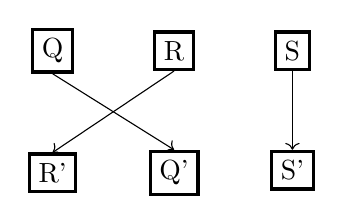
\begin{tikzpicture}
    [roundnode/.style={circle, draw=black, very thick},
    squarednode/.style={rectangle, draw=black, very thick},]

    %Nodes
    \node[squarednode](Q){Q};
    \node[squarednode](R)[right=of Q]{R};
    \node[squarednode](S)[right=of R]{S};

    \node[squarednode](Q')[below=of R]{Q'};
    \node[squarednode](R')[below=of Q]{R'};
    \node[squarednode](S')[below=of S]{S'};

    %Lines
    \draw[->](Q.south)--(Q'.north);
    \draw[->](R.south)--(R'.north);
    \draw[->](S.south)--(S'.north);
\end{tikzpicture}

        \caption{Voting pairs (the node being added, and the shielded blinding factor) will be permuted, so that only the MPC member will know which post sharded node corresponds to which pre-sharded node.}
        \label{fig:figure4}
\end{figure}

Once the threshold MPC has been conducted, nodes will be of the form
$$ g_is_2s_3P + r_{i,j,1}s_1s_2s_3P + r_{i,j,2}s_2s_3P, \hspace{2mm}r_{i,j,1}s_1s_2s_3P, \hspace{2mm} r_{i,j,2}s_2s_3P. $$

Now we can subtract the two to get out $g_is_2s_3P$. The previous values, $g_iP + r_{i,j,1}s_1P + r_{i,j,2}P$ were all different, but the returned values from each node are the same if they are from the same voter. Figure \ref{fig:figure5} provides a visual of what will be visible to an MPC member when contributing their final shard, as they will be the ones to uncover nodes from the same voter in their batch.

\begin{figure}[h!]
        \centering
        
   
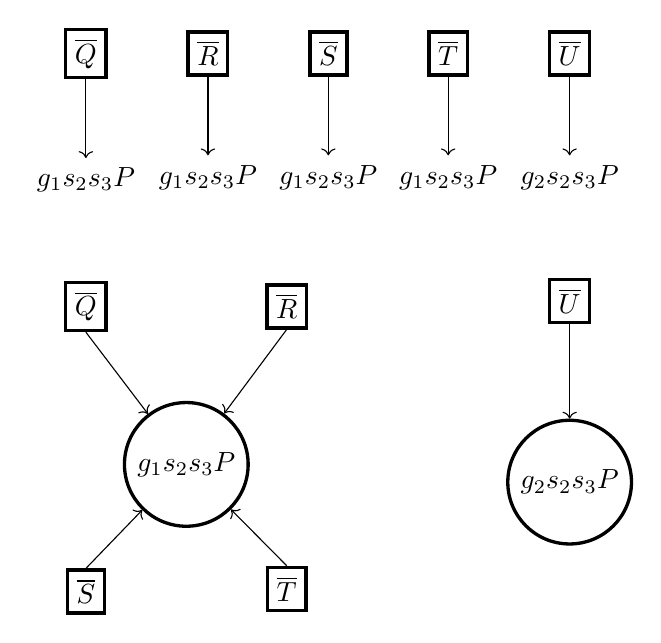
\begin{tikzpicture}
    [roundnode/.style={circle, draw=black, very thick},
    squarednode/.style={rectangle, draw=black, very thick},]

    %Nodes
    \node[squarednode](Q){$\overline{Q}$};
    \node[squarednode](R)[right=of Q]{$\overline{R}$};
    \node[squarednode](S)[right=of R]{$\overline{S}$};
    \node[squarednode](T)[right=of S]{$\overline{T}$};
    \node[squarednode](U)[right=of T]{$\overline{U}$};

    \node(q)[below=of Q]{$g_1s_2s_3P$};
    \node(r)[below=of R]{$g_1s_2s_3P$};
    \node(s)[below=of S]{$g_1s_2s_3P$};
    \node(t)[below=of T]{$g_1s_2s_3P$};
    \node(u)[below=of U]{$g_2s_2s_3P$};

    \node[squarednode](Q1)[below=of q]{$\overline{Q}$};
    \node[squarednode](R1)[right=2cm of Q1]{$\overline{R}$};
    \node[roundnode](node)[below=1.2cm of {$(Q1)!0.5!(R1)$}]{$g_1s_2s_3P$};
    \node[squarednode](S1)[below=3cm of Q1]{$\overline{S}$};
    \node[squarednode](T1)[below=3cm of R1]{$\overline{T}$};

    \node[squarednode](U1)[below=of u]{$\overline{U}$};
    \node[roundnode](node2)[below=1.2cm of U1]{$g_2s_2s_3P$};


    %Lines
    \draw[->](Q)--(q);
    \draw[->](R)--(r);
    \draw[->](S)--(s);
    \draw[->](T)--(t);
    \draw[->](U)--(u);

    \draw[->](Q1.south)--(node);
    \draw[->](R1.south)--(node);
    \draw[->](S1.north)--(node);
    \draw[->](T1.north)--(node);

    \draw[->](U1.south)--(node2);
\end{tikzpicture}

        \caption{This represents what is visible to an MPC member when they apply the final shard; they uncover which nodes in their batch are from the same voter.}
        \label{fig:figure5}
\end{figure}

On the last leg of the MPC, where each committee member applies the final shard, there will be a couple more tasks. Firstly, MPC members will unshield the pointer to see which votes are from the same voter. Secondly, they will run through their batch of revealed votes and remove duplicates without changing the vote (by reducing modulo the number of vote options).

For example, if there are 2 vote options, then if a vote subtree that they see has 5 votes, they will remove 4 of them and reveal 1. If there are 4 votes, they will remove 2 of them (we cannot reduce to 0 as that might remove the vote - the vote organiser will be free to decide if there is a null vote option). This way, the voter's choice is not changed, but the post-MPC trees will not be the same size as the pre-MPC trees, and this is a factor that helps prevent bribery and collusion. Figure \ref{fig:figure6} provides a visual of what will be visible to observers of the proof produced by an MPC member when the MPC member is the last contributor in the MPC to a batch.

\begin{figure}[h!]
        \centering
        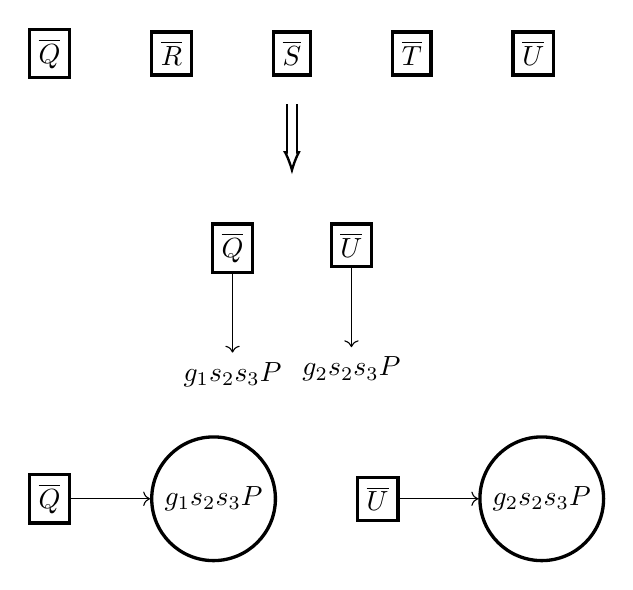
\begin{tikzpicture}
    [roundnode/.style={circle, draw=black, very thick},
    squarednode/.style={rectangle, draw=black, very thick},]

     %Nodes   
    \node[squarednode](Q){$\overline{Q}$};
    \node[squarednode](R)[right=of Q]{$\overline{R}$};
    \node[squarednode](S)[right=of R]{$\overline{S}$};
    \node[squarednode](T)[right=of S]{$\overline{T}$};
    \node[squarednode](U)[right=of T]{$\overline{U}$};

    \node(center-top)[below=0.1cm of S]{};
    \node(center-bottom)[below=0.9cm of center-top] {};

    \node[squarednode](Q2)[below left=0.5cm of center-bottom]{$\overline{Q}$};
    \node[squarednode](U2)[below right=0.5cm of center-bottom]{$\overline{U}$};

    \node(G1)[below=of Q2]{$g_1s_2s_3P$};
    \node(G2)[below=of U2]{$g_2s_2s_3P$};

    \node[squarednode](Q3)[below=5cm of Q]{$\overline{Q}$};
    \node[roundnode](node)[right=of Q3]{$g_1s_2s_3P$};
    \node[squarednode](U3)[right=of node]{$\overline{U}$};
    \node[roundnode](node2)[right=of U3]{$g_2s_2s_3P$};

    %Lines
    \draw[double distance=1mm, -{Latex[length=0.3cm,open]}, line width=0.3mm] (center-top) to (center-bottom);
    \draw [double distance=0.6mm, white, line width=0.2mm] (center-top) to ($(center-bottom)+(0,3.8mm)$);

    \draw[->](Q2)--(G1);
    \draw[->](U2)--(G2);

    \draw[->](Q3)--(node);
    \draw[->](U3)--(node2);
\end{tikzpicture}

        \caption{This represents what is visible to observers of the proof of the final MPC member on a batch. Any redundant nodes in a voting tree are discarded, so all voting trees uncovered publicly should contain between 1 and $o$ nodes, where $o$ is the number of options in the vote.}
        \label{fig:figure6}
\end{figure}

It was possible that a briber might ask a voter to create a vote tree with, for example, 513 edges - the absence of such a tree would leave the briber certain that the bribee did not do as requested. But if we remove these redundant nodes, then we prevent such a possibility. The only way to know the full trees at the end of the MPC would be to bribe every single member who took part in the MPC, a highly unrealistic possibility.

The post-MPC trees will now be visible (and they will have the same valency modulo the number of voter options), and due to the permutation, it will not be possible to see which post-MPC votes correspond to which pre-MPC votes. Moreover, due to the multiplication by the secret keys $s_1$ and $s_2$, nobody can determine any connections to entries in the accumulator either.

Note that none of the post-sharded nodes could be calculated by voters themselves, so there is no way to get a 'receipt' for your vote; i.e. there is no way to prove how you voted. A voter may reveal nodes that they created, but any viewer can have no certainty that the voter revealed all nodes they created.

As mentioned in the prerequisites, we can now tally our vote by determining the valency of the trees in the forest.

\section{Voting system properties}
The vote tallying is conducted in a decentralised manner, with no dependency on a trusted central entity for the tallying. There is still the involvement of the organisation to maintain the whitelist and initialise the vote, but this is usually going to be the case in any voting system.
When I find more time I will try to explain/argue why this mechanism has all of these properties (descriptions of these properties copied from \hyperlink{https://medium.com/privacy-scaling-explorations/release-announcement-maci-1-0-c032bddd2157}{this} MACI blog post).
\begin{itemize}
    \item Collusion resistant: no-one, except a trusted coordinator, can be convinced of the validity of a vote, reducing the effectiveness of bribery. (Voters can prove they voted for anything, so nobody can be convinced).
    \item Receipt-freeness: a voter cannot prove, besides to the coordinator, which way they voted (receipts for all possible results makes receipts redundant)
    \item Privacy: no-one, except a trusted coordinator, should be able to decrypt a vote (done via an MPC, so practically infeasible).
    \item Uncensorability: no-one, not even the trusted coordinator, should be able to censor a vote (once the organiser sends the initial records to initiate a vote, a voter cannot be suppressed online).
    \item Unforgeability: only the owner of a user’s private key may cast a vote tied to its corresponding public key (by design, as initial records are sent to the voters' public addresses, and revotes require proof of public key's membership in a whitelist).
    \item Non-repudiation: no-one may modify or delete a vote after it is cast, although a user may cast another vote to nullify it (provided by our system).
    \item Correct execution: no-one, not even the trusted coordinator, should be able to produce a false tally of votes (MPC requires agreement about which votes to tally, and this is deterministic if done honestly; and the maths of the tallying ensures it is done correctly).
\end{itemize}

We explain each of these points in further detail.
\subsection{Collusion Resistance and Receipt-Freeness }
In its traditional form, collusion resistance means that voters are unable to prove to any third party how they voted.  The third party is generally thought of as a corrupt actor trying to bribe individual voters.  Because any such actor would demand proof that the vote was cast in accordance with their arrangement before paying the bribe, a voting scheme that leaves no evidence with which to convince the bribing party is considered to be safe from such malicious interference.  This is why traditional polling locations do not generate receipts for voters to take home with them.  It is also one of the primary objections to mail-in voting, whereby a voter could theoretically mark, seal, and send in their ballot in front of a third party in exchange for payment.

We take a different approach to collusion resistance: rather than preventing voters from revealing their true vote, we provide them with the means to reveal \emph{any} vote.  By analogy to traditional polling locations, our system is akin to one in which voters leave the booth with receipts stating that they voted for each of the candidates.  The voter can then present the appropriate receipt to the corrupt third party and collect the bribe regardless of the actual vote they cast.  Of course, because it is common knowledge that voters have the means to prove any outcome they wish, the proof becomes meaningless and third parties do not try to bribe voters to begin with.  

This plays out in our system as follows: suppose that in a vote between $N$ candidates $C_0, C_1, \ldots C_{N-1}$ Alice wishes to vote for candidate $C_k$.  Recall that in the final tally, all of Alice's ballots will be counted and their number modulo $N$ will determine which candidate receives Alice's vote. So Alice could vote for $C_k$ simply by submitting $k$ ballots.  Now suppose that Alice has received an offer from Bob: 1 BTC if she votes for candidate $C_0$. Alice wishes to collect the 1 BTC from Bob and still vote for $C_k$ as she originally intended. Rather than submitting $k$ ballots, Alice submits $N+k$ ballots (or $2N+k$, or $3N+k$, etc.).  Each of Alice's ballots has the form $(g_A  P + r_{A,j,1} s_1 P, r_{A,j,1} s_2 P, r_{A,j,2}s_2P)$ for $j=1,2, \ldots N+k$. Bob sees all ballots cast by all voters, but due to their shielded form he cannot identify Alice's votes from among them.  Alice may, however, reveal any of her ballots to Bob by sharing with him a randomly generated number pair $r_{A,j,1}, r_{A,j,2}$ with which she shielded the ballot.  Bob then computes $r_{A,j,1} s_2 P$ and is convinced that Alice did indeed cast the given ballot because otherwise she would have had to solve a discrete logarithm problem to determine $r_{A,j,1}$ from the publicly visible EC point $r_{A,j,1}s_2 P$.  Bob now computes $r_{A,j,a} s_1 P$ and $r_{A,j,2}P$, and subtracts them from $g_A P + r_{A,j,1} s_1 P + r_{A,j,2}P$ to see the curve point $g_A P$.  If Alice reveals multiple votes to Bob, all will contain the same point $g_A P$, further convincing Bob that Alice has honestly revealed her votes to him.  

The crucial observation is that Alice may reveal \emph{as many of her votes} to Bob as she wishes, but he will have no way of knowing whether she has revealed \emph{all of her votes.}  So to prove to Bob that she voted for candidate $C_0$, Alice reveals $N$ of her ballots, leaving the remaining $k$ ballots shielded.  The DLP makes it impractical for Bob to try to unshield other ballots to see whether Alice left any hidden from him.  Bob realizes the futility of trying to bribe Alice and so he never tries in the first place.

This simple method of counting a voter's ballots modulo $N$ allows voters the option to convince a third party of anything they wish, thus rendering collusion nearly impossible.  Our tally is slightly more complex than simply counting ballots modulo $N$ to prevent the following sort of attack: Bob could pick a large integer $b$ and tell Alice that she will receive 1 BTC if she votes for $C_0$ by submitting precisely $bN$ ballots.  He will demand that she reveal all $bN$ ballots to him.  To convince himself that Alice did not submit any more than $bN$ ballots, Bob will check the output of the final tally to verify that there is a tree with precisely $bN$ leaves.  If no such tree is present, Bob knows that Alice has broken their agreement.  Since all computations are performed over a field of large order, the probability of another voter having submitted precisely $bN$ votes when Alice herself submitted $bN+k$ votes is low, and so Alice's probability of successfully deceiving Bob is negligible.  Thus the final tally must not reveal the sizes of all trees, as this information could be used to enforce the conditions of a bribe.  This motivates the intermediate step in our MPC where each tree is trimmed to a length of between $1$ and $N$ without changing its size modulo $N$.  In this step the information that Bob would have used to enforce the bribe is thrown away, again rendering collusion impossible.  We ensure integrity in the form of a zero-knowledge proof that the initial and final sizes of the tree are congruent modulo $N$.

Note that receipt-freeness is achieved by giving voters the option to prove any possible outcome.  Thus receipt-freeness is achieved by giving away so many receipts that any individual one becomes meaningless.  It is precisely via this property that we achieve collusion resistance.

\subsection{Privacy}


\section{Performance}
Let's say voters will be producing a 

Let's say that there are $b$ batches, each with $d$ nodes. Each MPC member, when conducting their step of the MPC, will need to create a SNARK that proves:
\begin{itemize}
    \item They applied their shard of $s_1s_3$ correctly (using the same shard each time)
    \item They applied their shard of $s_2s_3$ correctly (using the same shard each time)
    \item They applied their shard of $s_2s_3$ correctly (using the same shard each time)
    \item They permuted their batch of votes
\end{itemize}

The EC multiplication cost is of course linear in $d$ (with windowed multiplication costing around 3 constraints per bit), and the permutation under an R1CS setting can be done in around $n\log_2(n)-n$ switches (where a single 2x2 switch costs 2 constraints).

This needs more thinking about what happens in which fields and where the constraint numbers should come from. If voters need to prove that they encrypted their vote correctly, then maybe the proofs of the MPC members will need to be on a chained curve?

Let's say we use the 2-chain BLS12-377 and BW6-761 (the scalar field of the latter is the base field of the former), then the EC points that are output as nodes by voters should consist of 377 bits. Each EC multiplication should be possible in around 3 constraints per bit, yielding around 1131 constraints; and therefore around 2262 constraints for multiplication per voter node. Note that multiplication requires a binary decomposition for the multiplying scalar, but since we only use 2 scalars for multiplying ($s_1$ and $s_2$), this cost is amortised.

This yields a rough cost per committee member of
$$ 2262*d + 2d\log_2(d) - d = 2263d + 2d\log_2(d)
$$ 
constraints. A batch size of $10,000$ would thus yield around $22,910,000$ ($23$ million) constraints, and this might take up to .... to produce a proof of.

Depending on the computational power of the MPC members we might expect, we can have batch sizes if up to ....

There is one additional performance to look at, and this is the final step of the MPC because it involves all of the steps above, but it also involves a removal of repeated elements. This additional step might involve somewhere in the region of ......


\section{Use cases}
This system can be used as pleased, but the original thinking is that it would be a 1 voter 1 vote type system. 

Verifiable credentials could be used to safely build up a list of eligible voters. For example once we have the infrastructure to prove that Binance did KYC and approved you as person X, then you can use that to prove your validity. There are other options, but this is a useful possibility.

\section{Next steps}
There are a few things in this that require more thought/work. Ideas from anybody would be welcome
\begin{enumerate}
    \item A rough upper bound on the number of nodes within a batch
    \item A projection on how long the MPC (vote tallying would take)
    \item Which accumulator schemes would make sense to use with this system
    \item Discussion of the issue of selling a private key. Perhaps there is a way to remove the possibility of determining a vote even with the private key; maybe this could be done via nullifiers and sending records to the vote tallying public key?
    \item It is important to consider in more detail how MPC committee members will be selected and the committee updated. It would be unwise to have the organisation create and share the key, but how committee members will be selected is of importance (though fortunately even if they are corrupt the worst case scenario is that they will be able to see how people voted - they will not be able to create votes)
    \item Should add the possibility for turning the vote into nothing too (i.e. add an option that is a null vote)
\end{enumerate}

\section{Potential problems}
Sybil attack. Perhaps something that will help reduce this is the inclusion of PoW. i.e. for each vote a nonce has to be added such that when hashed with the voting info, we will get $x$ number of zeros (alternatively make a vote record cost a euro). Maybe make it take an hour to find? Also, if used at more important scales, perhaps physical hardware could be required to vote too (similar to a card reader for banking transactions).

If the MPC committee work together they can also determine which original vote a Sybil attack came from. The committee can decide to try to uncover this if they wish for slashing purposes. However the committee will not know the identity of the voter, they will only be able to see some of the voting records. Providing this information to O will allow O to determine their identity.

\section{Acknowledgements}
We would like to say a big thanks to Kobi Gurkan for providing thoughts and pointing out weaknesses in several iterations of this design. A thanks also to Pratyush Mishra for helping understand some of the computational limitations to the design that led to many simplifications being discovered.

\section{Appendix}
\subsection{Threshold encryption}
We will not discuss here how the keys can be created in a decentralised, non-interactive manner; you can see all the details in \href{https://eprint.iacr.org/2021/339.pdf}{Groth}. The setup creates a polynomial 
$$f(x) = \sum_{i=0}^{k-1}c_ix^i$$ and distributes evaluations of this polynomial at different points to nodes. We will only focus on how the threshold encryption works.

Evaluating the polynomial $f(x)$ at $0$, yielding $f(0) = c_0$ provides the secret key (i.e. $s = c_0 = f(0)$). We can calculate $sP$ from $P$ and shards of this polynomial without anybody learning $s$ via a threshold MPC.

The shards that the nodes have are evaluations of this polynomial at different points. Let's say there are $n$ nodes with shards, then node $j$ has the shard $f(j) = \sum_{i=0}^{k-1}c_ij^i$. (in practise, node $j$ does not necessarily need to have the evaluation at $j$, but it simplifies the description).

Let's say $k$ of the nodes get together and share their indices with each other (call their index set $U$). Then they can create Lagrange polynomials $L_i(x)$ - i.e. polynomials that evaluate to zero at all indices of the other nodes, and evaluate to $f(j)$ for their node (i.e. $L_i(x) = 0 \hspace{2mm} \forall j \in U\backslash\{i\}$ and $L_i(i) = f(i)$.

If each of these nodes calculates $L_i(x)$ and add their results together to get $g(x)=\sum_{i\in U}L_i(x)$, it turns out this sum will be equal to $f(x)$. This is because $g(x)$ will be a $k-1$ degree polynomial (by construction), and we also have that $f(i)=g(i)$ for all $i\in U$. Any polynomials of degree $m$ whose evaluations at at least $m+1$ points are equal must actually be the same polynomial.

Thus, if each of these nodes evaluates $L_i(0)$ and add their results together to get $\sum_{i\in U}L_i(0)$, what we will actually have is $g(0)=f(0)=s$.

Hence if node $1$ takes in $P$ and produces $L_1(0)P$, then node $2$ can calculate $(L_1(0)+L_2(0))P$. Continuing this, we will eventually get
$$\sum_{i\in U}L_i(0)P = sP$$ As a note, it is possible to do this MPC in a verifiable manner; this can be discussed later.

\end{document}
